\documentclass{article}
\usepackage{hyperref}
\usepackage{vmargin}
\usepackage{amsmath}
\usepackage{graphicx}
\setpapersize{USletter}
\setmarginsrb{1in}{1in}{1in}{1in}{0.25in}{0.25in}{0in}{0in}

\newcommand{\comment}[2]{[{\Large\sc #1:} \textsf{#2}]}

\newcommand{\doug}[1]{\comment{Doug}{#1}}
\newcommand{\gary}[1]{\comment{Gary}{#1}}
\newcommand{\jaakko}[1]{\comment{Jaakko}{#1}}

\begin{document}

\markboth{Doc. no: N1704=04-0144}{Doc. no: N1704=04-0144}
\pagestyle{myheadings}

\title{Variadic Templates: Exploring the Design Space}
\author{Douglas Gregor \and Jaakko J\"arvi \and Gary Powell}
\date{}
\maketitle

\par\noindent Document number: N1704=04-0144
\par\noindent Revises document number: N1603=04-0043
\par\noindent Date: \today
\par\noindent Project: Programming Language C++, Evolution Working Group
\par\noindent Reply-to: Douglas Gregor $<${\tt gregod@cs.rpi.edu}$>$

\section{Introduction}
This proposal directly addresses two problems:
\begin{itemize}
\item The inability to instantiate class and function templates with an arbitrarily-long list of template parameters.
\item The inability to pass an arbitrary number of arguments to a function in a type-safe manner.
\end{itemize}

The proposed resolution is to introduce a syntax and semantics for
variable-length template argument lists (usable with function templates
via explicit template argument specification and with class templates)
along with a method of argument ``packing'' using the same mechanism to
pass an arbitrary number of function call arguments to a function in a
typesafe manner.

\section{Motivation}
\subsection{Variable-length template parameter lists}
Variable-length template parameter lists (variadic templates) allow a
class or function template to accept some number (possibly zero) of
template arguments beyond the number of template parameters specified.
This behavior can be simulated in C++ via a long list of defaulted
template parameters, e.g., a typelist wrapper may appear as:

\begin{verbatim}
struct unused;
template<typename T1 = unused, typename T2 = unused, 
         typename T3 = unused, typename T4 = unused, 
         /* up to */ typename TN = unused> class list;
\end{verbatim}

This technique is used by various C++ libraries~\cite{Tuples01,
Jarvi02, Gurtovoy02}. Unfortunately, it leads to very
long type names in error messages (compilers tend to print the
defaulted arguments) and very long mangled names. It is also not
scalable to additional arguments without resorting to preprocessor
magic~\cite{Preprocessor01}. In all of these libraries (and presumably
many more), an implementation based on variadic templates would be
shorter and would not suffer the limitations of the aforementioned
implementation. The declaration of the {\tt list<>} template above may
be:
\begin{verbatim}
template<... Elements> class list;
\end{verbatim}

\subsection{Typesafe Variable-length Function Parameter Lists}
Variable-length function parameter lists allow more arguments to be
passed to a function than are declared by the function. This feature
is rarely used in C++ code (except for compatibility with C
libraries), because passing non-POD types through an ellipsis ({\tt
  ...}) invokes undefined behavior. However, a typesafe form of such a
feature would be useful in many contexts, e.g., for implementing a
typesafe C++ {\tt printf} that works for non-POD types.

\section{Feature menu}
Prior versions of this proposal~\cite{GPJ03,GJP04a} described various
points in the design space of variadic templates. In this version of
the proposal, we have chosen to enumerate the various potential design
decisions (mainly features) and discuss the impact of each on users
and compilers. Fig.~\ref{fig:dependencies} illustrates the
dependencies between features, such that an edge $A \rightarrow B$
indicates that feature $A$ requires acceptence of feature $B$.

\begin{figure}
\center
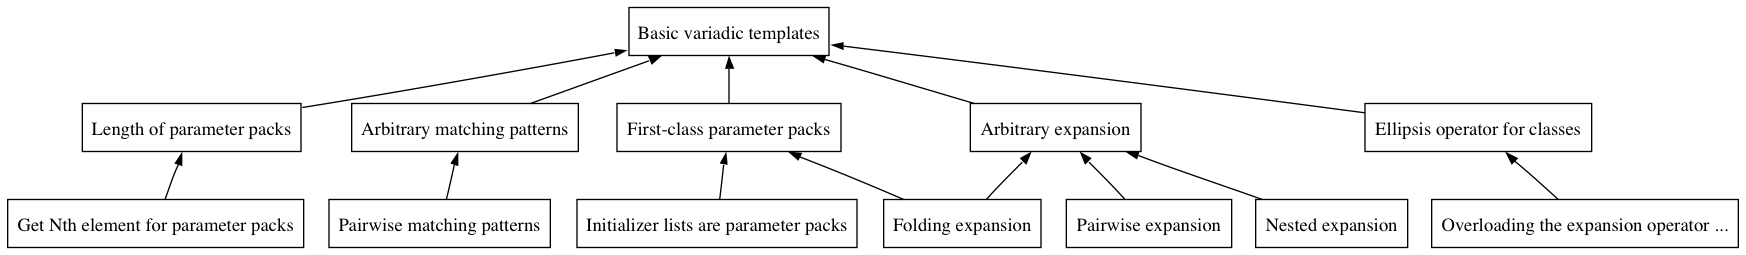
\includegraphics[width=6in,height=3in]{vt_deps}
\caption{Feature dependency graph for variadic templates}
\label{fig:dependencies}
\end{figure}

The following sections describe each feature listed in
Fig.~\ref{fig:dependencies}. Sec.~\ref{sec:specials} then provides several
``specials'': prepacked sets of features that work well together and
represent some overall goal for variadic templates. It is our hope
that the committee will select a special or a set of features
\textit{a la carte} for which we can draft a more formal
specification. 

\subsection{Basic variadic templates}
\label{sec:basic}
The most basic form of variadic templates requires the ability to
declare class/struct/union and function templates that accept an
arbitrary number of template arguments, declare function templates
that accept an arbitrary number of (function) arguments, and access
the ``extra'' template and function arguments.

We adopt the use of the ellipsis operator ``\texttt{...}'' to
represent variable-length argument lists. For variadic class templates
we allow ``\texttt{...}'' as the ``kind'' of the last template
parameter, which may optionally be followed by an identifier. The
following class template accepts one type argument followed by zero or
more other template arguments.

\begin{verbatim}
template<typename T, ... Tail> class tuple;

typedef tuple<int, float, double, std::string, 5, std::vector> t;
\end{verbatim}

Variadic function templates are declared similarly, allowing one to
explicitly specify any number of arguments:
\begin{verbatim}
template<... Args> void print_template_args();

print_template_args<int, 17, 42.0, &X::m>();
\end{verbatim}

We refer to \texttt{Tail} and \texttt{Args} as ``template parameter
packs'', because they pack together a set of template arguments into a
single parameter. In their most basic form, template parameter packs
provide only a single operation: unpacking via the ellipsis
(\texttt{...}) operator). Unpacking splits a template parameter pack
into its individual arguments, allowing each to be considered
individually. For instance, the following code builds a recursive
tuple from the types given:
\begin{verbatim}
template<typename Head, ... Tail> struct tuple { // #1
  Head head;
  tuple<Tail...> tail;
};

template<typename Head> struct tuple<Head> { // #2
  Head head;
};
\end{verbatim}

The instantiation of \texttt{tuple<int, double, std::string} uses the
primary template (\#1) with \texttt{Head}=\texttt{int} and
\texttt{Tail} containing \texttt{double} and \texttt{std::string},
which we denote by \texttt{Tail}=\texttt{<double, std::string>}. The
\texttt{tail} member is a tuple that will receive the template arguments
\texttt{double} and \texttt{std::string}, in that order, due to the
application of the \texttt{...} operator to the template parameter
pack \texttt{Tail}. 

The ellipsis operator represents both unpacking and packing arguments,
depending on context. For instance, a partial specialization can fix
some number of arguments and collect the rest in a template parameter
pack:

\begin{verbatim}
// Searching for two adjacenct types...
template<typename T, ... Elements> 
struct adjacent_find : adjacent_find<Elements...> { };

// Found adjacenct types!
template<typename T, ... Rest>
struct adjacent_find<T, T, Rest...> {
  static const bool value = true; 
  typedef T type;
};

// List is empty. We found nothing.
template<> struct adjacent_find { static const bool value = false; };
\end{verbatim}

Here, the partial specialization matches the case where two adjacent
types are the same and then collects the rest of the arguments into
the template parameter pack \texttt{Rest}. The ellipsis operator can
be applied to a parameter pack wherever there is a list of parameters
(for packing) or arguments (for unpacking), including:
\begin{itemize}
  \item In a partial specialization (e.g., the \texttt{adjacent\_find} example)
  \item In a \textit{template-id} (e.g., \texttt{tuple<Elements...>})
  \item In a function type (e.g., \texttt{void(int, ArgTypes...)})
\end{itemize}

The ellipsis operator also applies to \textit{value} parameter packs,
which store run-time values for type-safe variadic function
templates. For instance, a type-safe \texttt{printf} might be declared
as:

\begin{verbatim}
template<... Args> void printf(const char* s, const Args& args...);
\end{verbatim}

This declaration indicates that \texttt{printf} accepts a variable
number of parameters (both template and function arguments): the
\texttt{Args} template parameter pack contains the types of the
arguments, whereas the \texttt{args} template parameter pack contains
the values. The ellipsis operator following ``\texttt{args}''
indicates that extra arguments to \texttt{printf} should be bundled
into the \texttt{args} parameter pack and their types deduced and
placed into the \texttt{Args} template parameter pack. In this basic
version, the template parameter pack containing the types of the
arguments may be a \textit{cv}-qualified template parameter pack or a
reference to a \textit{cv}-qualified template parameter pack. 

One can think of the typesafe variadic \texttt{printf} function as
having an expansion to a family of overloads each having a different
number of arguments:

\begin{verbatim}
void printf(const char* s);
template<typename T1> void printf(const char* s, const T1& a1);
template<typename T1, typename T2> 
  void printf(const char* s, const T1& a1, const T2& a2);
/* up to some arbitrary N */
template<typename T1, typename T2, /* up to */, typename TN> 
  void printf(const char* s, const T1& a1, const T2& a2, /* up to */, const TN& aN);
\end{verbatim}

The most basic formulation of variadic templates therefore consists
of:
\begin{itemize}
\item The ability to declare template and value parameter packs
\item The ability to unpack and pack template and value parameter
  packs via the ellipsis operator.
\item Partial ordering rules for class template partial
  specializations and function templates in the presence of variadic
  templates (discussed in a previous proposal~\cite{GJP04a}).
\end{itemize}

\subsection{First-class parameter packs}
\label{sec:first-class-pp}
In the basic formulation, template and value parameter packs are
merely bundles of parameters that have no direct representation within
the type system. However, we could make template parameter packs into
actual types---albeit special ones that permit the use of the ellipsis
operator---so that they could be passed to template arguments or
compared against each other. Moreover, value parameter packs now have
actual types based on the type of the associated template parameter
pack, and may become first-class objects templates. Thus they can be
default-constructed (if all types in them are default-constructible),
copy-constructed or assigned (if all types of copy-constructible or
assignable, respecitvely), and unpacked as needed. 

First-class parameter packs have some advantages over the basic
formulation of parameter packs, because it allows multiple arguments
to be stored together without resorting to recursion as with the
\texttt{tuple} template in Sec.~\ref{sec:basic}:
\begin{verbatim}
template<... Elements> 
class tuple
{
public:
  tuple(const Elements& elements...) : elements(elements) { }

private:
  Elements elements;
};
\end{verbatim}

Here we store members of every type in \texttt{Elements} in a single
parameter pack within the tuple, instead of creating a chain of
\texttt{tuple} instantiations where each stores a single element plus
the next \texttt{tuple} in the chain. 

\paragraph{User impact}: First-class parameter packs make writing some
heterogenous data structures simpler because they can eliminate the
need for recursive data structures. Performance (both compiler and
generated code) will improve because the number of instantiations
required to implement a heterogeneous data structure will be reduced
from ${\cal O}(N)$ to ${\cal O}(1)$. This effect has already been seen
when comparing the Boost.Tuples library~\cite{Tuples01}, which uses a
recursive data structure, to a preprocessor-based library, which
enumerates all data members. 

First-class parameter packs may be somewhat confusing to users,
because the distinction between a ``packed'' parameter pack and an
unpacked one becomes very important. For instance, if one forgets to
apply the ellipsis operator the compiler will pass the parameter pack
itself, e.g.,
\begin{verbatim}
template<... Args> void debugout(const std::string& s, const Args& args...)
{
  printf(("Debug: " + s).c_str(), args); // oops, should be "args..."
}
\end{verbatim}

\paragraph{Compiler impact}: First-class parameter packs introduce
more complexity into the implementation of variadic templates, because
the compiler must construct actual types and objects for each
parameter pack. In addition, there are some interesting interactions
between the object model used for parameter packs and the method by
which arguments are passed to function objects that require further
consideration; see~\cite{GJP04a}. 

\paragraph{Evaluation}: The most important realization with
first-class parameter packs is that they can be emulated via recursive
data structures. However, this emulation places an extra burden on
users and compilers, and is known to result in poorer performance.

\subsection{Initializer lists are parameter packs}
Initializer lists are typeless entities stored in the compiler that
can only be used in very restrictive ways for initializing
aggregates. We could lift some of the restrictions on initializer
lists by making them (value) parameter packs. This would permit writing
constructors and assignment operators that accept initializer lists,
e.g.,

\begin{verbatim}
template<... Elements>
class tuple
{
public:
  // #1: Build from an initializer list
  tuple(Elements elements) : elements(elements) { }

  // #2: Build from an initializer list, converting as necessary
  template<... Args> tuple(Args args) : elements(args...) { }

private:
  Elements elements;
};

// Passes initializer list as parameter pack to constructor #1
tuple<int, double, float> t1 = { 17, 3.14159, 2.718f };
  
// Passes initializer list as parameter pack to constructor #2
tuple<int, double, std::string> t2 = { 17, 3.14f, "foo" };
\end{verbatim}

Additionally, this change permits emulation of sequence
constructors~\cite{DoReStr03} via parameter packs, e.g.,
\begin{verbatim}
template<typename T>
class vector
{
public:
  template<... Elements> vector(Elements elements)
  {
    tr1::array<T, (pp_length<Elements>::value)> a = elements;
    assign(a.begin(), a.end());
  }
};
\end{verbatim}

The construction of \texttt{a} actually performs aggregate
initialization from the incoming parameter pack, which unfortunately
requires one extra copy. This copy can be elided by implementing the
constructor as a metaprogram\footnote{See Sec.~\ref{sec:pp-size} for a
  discussion of \texttt{pp\_length}}:

\begin{verbatim}
template<typename T>
class vector
{
public:
  template<... Elements> vector(const Elements& elements)
  {
    reserve(pp_length<Elements...>::value);
    do_push_back(elements...);
  }

  void push_back(const T&);

private:
  template<... Rest>
  void do_push_back(const T& x, Rest... rest) {
    push_back(x);
    do_push_back(rest...);
  }

  void do_push_back() {}
};
\end{verbatim}

\paragraph{User impact}: The ability to accept initializer lists in
the constructors and assignment allows us to make initialization of
standard library data structures (and other user types) more natural,
and may improve readability of the language. It also subsumes several
of the ideas in~\cite{DoReStr03}.

\paragraph{Compiler impact}: Implementation of this feature is not
expected to require a great deal of effort beyond that of implementing
first-class parameter packs because the extension is small and pure.

\subsection{Ellipsis operator for classes}
One extension of the ellipsis operator would permit it to be applied
to any object of class type, which would have the effect of unpacking
all of the fields in that class type into separate arguments. This
information could be used for compile-time reflective metaprogramming,
e.g., to perform automatic marshalling or to construct property
inspectors. 

\paragraph{User impact}: While we do not expect that many users would
apply the ellipsis operator to classes, there are many secondary
benefits to users when library developers are able to apply reflection
to provide features that typically require preprocessing or user
intervention. 

\paragraph{Compiler impact}: Implementation of this feature could
require a moderate amount of work depending on the format used to
describe the members of the class. We have not considered such a
format in depth.

\subsection{Overloading the expansion operator ...}
This proposal introduces \texttt{...} as a full-fledged operator only
usable for special, compiler-defined parameter packs. Some
user-defined types (notable the library-defined \texttt{tuple} type)
may wish to present a parameter-pack---like interface and support the
ellipsis operator. \texttt{operator...} could be a nonstatic member
function taking zero arguments and returning a parameter pack. For
instance, within the \texttt{tuple} type:

\begin{verbatim}
template<... Elements>
  class tuple 
  {
    // ...
  public:
    Elements operator...() const { return elements; }

  private:
    Elements elements;
  };
\end{verbatim}

The ability to overload the ellipsis operator for any class type may
require a new syntax for unpacking, because it will be unclear which
objects are being unpacked. Consider:

\begin{verbatim}
template<typename T, typename U>
void foo(T t, U u)
{
  f(g(t, u), ...);
}
\end{verbatim}

In this case, we do not know which object (\texttt{t} or \texttt{u})
will be unpacked because either (or both) may have an overloaded
ellipsis operator. Having an overloadable ellipsis operator with this
syntax can make the ellipsis operator unusable in generic code.

\paragraph{User impact}: By allowing user data types to overload the
ellipsis operator, users may achieve more natural syntax for certain
types of data. On the other hand, the ambiguities introduced by the
ability to overload this operator may outweigh its advantages.

\paragraph{Compiler impact}: Implementation of this feature is expected to
require moderate effort, because it introduces another overloadable
operator and ambiguities with the expansion of parameter packs and
parameter pack-like types.

\subsection{Length of parameter packs}
\label{sec:pp-size}
One can determine the number of elements in a template parameter pack
with the following template:
\begin{verbatim}
template<...> struct pp_length;

template<typename T, ... Rest>
struct pp_length<T, Rest...> {
  static const int value = 1 + pp_length<Rest...>::value; 
};

template<> struct pp_length<> {
  static const int value = 0;
};
\end{verbatim}

However, this requires ${\cal O}(N)$ instantiations for a parameter
pack of length $N$, which can be inefficient to compile. This option
proposed that unpacking a template or value parameter pack in a
\texttt{sizeof} expression will return its length, e.g.,

\begin{verbatim}
template<... Args>
  void f(Args args...)
  {
    const int num_args = sizeof(args...);
    // equivalent to...
    const int num_args = sizeof(Args...);
  }
\end{verbatim}

\paragraph{User impact}: This feature gives users a simple, efficient
way to determine the length of a parameter pack. The absence of this
feature negatively affects both compile-time performance and usability.

\paragraph{Compiler impact}: This feature should be trivial to implement.

\subsection{Get Nth element for parameter pack}
Parameter packs are only accessible linearly, by peeling off arguments
at the front of the parameter pack. A general tuple, however, requires
the ability to access the $N^{\text{th}}$ element. For parameter
packs, we would like to be able to access the Nth element. For this we
propose to use the \texttt{[]} operator, but restrict the argument to
integral constant expressions because the result type differs
depending on the value of the argument. For instance,

\begin{verbatim}
template<... Args>
  void f(Args args)
  {
    // Make copy of 2nd argument
    decltype(args[1]) second = args[1];
  }
\end{verbatim}

We rely on \texttt{decltype}~\cite{JarviStroustrup04} to determine the
type of the $N^{\text{th}}$ argument. If \texttt{decltype} is not
accepted into C++0x, we would require additional syntax to extract the
$N^{\text{th}}$ argument from a template parameter pack in ${\cal
  O}(1)$ instantiations.

\paragraph{User impact}: This feature gives users a simple, efficient
way to access a value in the parameter pack. The absence of this
feature negatively affects both compile-time performance and usability.

\paragraph{Compiler impact}: This feature should be trivial to
implement.

\subsection{Arbitrary expansion}
With basic variadic templates, the ellipsis operator may only be
applied to a parameter pack. A more powerful form of the ellipsis
operator allows the parameter pack to occur within an expression of
arbitrary complexity followed by an ellipsis; in this case, expansion
is performed by replacing parameter pack with each of its values and
duplicating the expression for each value. Fig.~\ref{fig:expansions}
illustrates the expansions of several template and value parameter
packs. In the figure, \texttt{X} is a template parameter pack
containing template parameters \texttt{X1}, \texttt{X2}, ....,
\texttt{XN} and, when all \texttt{Xi} are types, \texttt{x} is a value
parameter pack of type \texttt{X} such that \texttt{x1}, \texttt{x2},
..., \texttt{xN} are the contained values. Similarly, \texttt{Y} is a
template parameter pack of size \texttt{M}, with associated
\texttt{Yi}, \texttt{y}, and \texttt{yi}. Additionally, assume the
following declarations:
\begin{verbatim}
template<...> class list;
template<...> class vector;
template<... Args> void f(Args args...);
template<... Args> void g(Args args...);
\end{verbatim}

\begin{figure}[h]
\centering
\begin{tabular}{l|l}
\textbf{Types \& Expressions} & \textbf{Expansion} \\\hline
\texttt{list<X...>} & \texttt{list<X1, X2, /* up to */, XN>} \\
\texttt{list<int, X..., float>} & \texttt{list<int, X1, X2, /* up to */, XN,
  float>} \\
\texttt{f(x...)} & \texttt{f(x1, x2, /* up to */, xN)} \\
\texttt{f(17, x..., 3.14159)} & \texttt{f(17, x1, x2, /* up to */, xN,
  3.14159)} \\
\texttt{int (*)(X...)} & \texttt{int (*)(X1, X2, /* up to */, XN)} \\
\texttt{list<typename add\_pointer<X>::type...>} &
\texttt{list<typename add\_pointer<X1>::type,} \\
& \qquad\texttt{{ }typename add\_pointer<X2>::type,} \\
& \qquad\texttt{{ }typename add\_pointer<XN>::type>} \\

\texttt{f(x*x)} & \texttt{f(x1*x1, x2*x2, /* up to */, xN*xN)} \\
\end{tabular}
\caption{Illustration of the expansions of types and
  expressions using template and value parameter packs.}
\label{fig:expansions}
\end{figure}

\paragraph{User impact}: Arbitrary expansions provide the equivalent
of a metaprogramming \texttt{transform} operation, that allows one
parameter pack to be transformed into another by applying some
function to each value. We expect that many users that need variadic
templates will also need arbitrary expansion.

\paragraph{Compiler impact}: Arbitrary expansions are clearly more
complicated to support than basic expansions, because they require the
compiler to store the expression (or type) patterns and produce a
sequence of expressions (or types) from those patterns. The
implementation is expected to be very similar to that of template
instantiation.

\paragraph{Evaluation}: Arbitrary expansions are very useful for
metaprogramming with parameter packs, but they are not absolutely
essential: one can construct these operations given only the basic
variadic templates, but they will require ${\cal O}(N)$ instantiations
instead of ${\cal O}(1)$ instantiations.

\subsection{Nested expansion}
With this feature, ellipses operators may be nested, with each
ellipsis binding to the argument text it follows. The same parameter
pack may appear in multiple places within the argument text (and all
will be replaced with the same type or argument from the parameter
pack in each expansion). 

The need for nested expansion is apparent when considering the
construction of a facility such as Bind~\cite[\S
  3.3]{Austern04b}. With this facility, there is a binder function
object consisting of a function object \texttt{f} and a set of bound
arguments $a_1, a_2, \ldots, a_n$ that has been passed actual
arguments $v_1, v_2, \ldots, v_m$. The bound arguments $a_i$ consist
of either (a) a value to be passed to \texttt{f}, (b) a placeholder
referring to one of the values $v_k$, or (c) another binder function
object. Thus, for each argument $i$ to \texttt{f} we need to consider
the bound argument $a_i$ and potentiall all actual arguments $v_k$. We
therefore define a function $\mu(a_i, v_1, v_2, \ldots, v_m)$ that
performs the mapping for each $a_i$. If \texttt{a} is a parameter pack
containing $a_1, a_2, \ldots a_n$ and \texttt{v} is a parameter pack
containing $v_1, v_2, \ldots, v_m$, we can implement the binder
function object's call to \texttt{f} via:

\begin{verbatim}
return f(mu(a, v...)...);
\end{verbatim}

This line of code first expands the inner ellipsis for \texttt{v} in
the call to \texttt{mu}, resulting in \texttt{mu(a, v1, v2, /* up to
  */, vm)}. Then the outer ellipsis is expanded for \texttt{a},
resulting in:
\begin{verbatim}
return f(mu(a1, v1, v2, /* up to */, vm),
         mu(a2, v1, v2, /* up to */, vm),
         /* up to */
         mu(an, v1, v2, /* up to */, vm));
\end{verbatim}

\paragraph{User impact}: This feature follows solidly in the category
``When you need it, you \textit{really} need it'', but will likely not
see widespread use. The lack of this feature will result in a great deal
of template metaprogramming require ${\cal O}(m \cdot n)$ instantiations.

\paragraph{Compiler impact}: Implementation of this feature is
expected to be relatively simple, requiring only that expansions be a
recursive operation.

\subsection{Pairwise expansion}
Arbitrary expansion requires that only a single parameter pack occur
within the pattern. Nested expansion extends this notion to several
parameter packs so long as the expansions are nested. Pairwise
expansion, on the other hand, allows two or more parameter packs at
the same nesting level so long as all parameter packs are of the same
length $N$. In this case, the parameter packs are expanded together
into $N$ arguments, with the $i^{\text{th}}$ argument having replaced
each parameter pack with the $i^{\text{th}}$ value in that parameter
pack.

Pairwise expansion permits, among other things, ``zipping'' two
parameter packs into a single parameter pack containing
pairs\footnote{Note that we also take advantage of first-class
  parameter packs in this example}:

\begin{verbatim}
template<... Args> struct bundle_t { typedef Args type; };

template<... Args> Args bundle(const Args& args...) { return args; }

template<... Args1>
class zipper
{
public:
  zipper(const Args1& args1...) : args1(args1) {}

  template<... Args2>
  typename bundle_t<std::pair<Args1, Args2>...>::type
  operator()(const Args2& args2...)
  { return bundle(std::pair<Args1, Args2>(args1, args2)...); }

private:
  Args1 args1;
};
\end{verbatim}

More importantly, pairwise expansion in conjunction with move
semantics~\cite{Hinnant02} permits perfect argument
forwarding~\cite{Dimov02} for an arbitrary number of
arguments\footnote{Additionally, we use \texttt{decltype} to provide
  perfect forwarding of the return type}:

\begin{verbatim}
template<typename F, ... Args>
auto apply(F&& f, Args&& args...) -> decltype(f(static_cast<Args&&>(args)...))
{ return f(static_cast<Args&&>(args)...); }
\end{verbatim}


%Finally, pairwise expansion gives a much more literal meaning to the
%declaration of the parameter packs in typesafe variadic functions, e.g.,
%
%\begin{verbatim}
%template<... Args> void foo(const Args& args...);
%\end{verbatim}
%
%Here, the 

\paragraph{User impact}: This feature is extremely important in
conjunction with the move semantics proposal~\cite{Hinnant02},
providing perfect argument forwarding. 

\paragraph{Compiler impact}: Implementation of this feature is
expected to be easy, requiring only that the compiler
be able to substitute for several parameter packs at once.

\subsection{Arbitrary matching patterns}
last...feature...here...

\section{Revision history}
\begin{itemize}

\item \textbf{Since N1603=04-0043}:
  \begin{itemize}
  \item Moved to feature-based decomposition of the variadic templates
    design space.
  \end{itemize}

\item \textbf{Since N1483=03-0066:} 
  \begin{itemize}
  \item Variadic templates no longer solve the forwarding problem for
    arguments. 
  \item Parameter packs are no longer tuples; instead, they are a
    compiler-specific first-class entities.
  \item Introduced the ability to deduce a template parameter pack
    from a type (or list of template parameters).
  \item Eliminated the \texttt{apply}, \texttt{integral\_constant},
    and \texttt{template\_template\_arg} kludges.
  \end{itemize}
\end{itemize}

\section{Acknowledgements}
Discussions among Daveed Vandevoorde, David Abrahams, Mat Marcus, John
Spicer, and Jaakko J\"arvi resulted in the new syntax for unpacking
arguments using ``...''. This proposal has been greatly improved with
their feedback. Mat Marcus suggested that the ellipsis operator could
be applied to class types for marshalling, reflection, etc. David
Abrahams noticed that ``...''  could be used for metaprogramming if we
supported arbitrary expansion patterns.

\bibliographystyle{abbrv}
\bibliography{template_varargs}
\end{document}
